\documentclass{article}
\usepackage[margin=20mm]{geometry}
\usepackage[T1]{fontenc}
\usepackage{tikz}
\begin{document}
\section*{Bounded symbol lifetime in canonical Core IR}
Created-at: 2026-09-25 04:05 +02:00. ETA 30--45 minutes: one shared visitor,
focused regressions, producer rebuild, live repair and validation.
\paragraph{Authorization} User: \textit{Engedély megadva a javításra} at03:56; the previous
plan-only decision is superseded. Core remains the single semantic authority.
\paragraph{Failure} HIVE43540:1085 declarations,65535 interned strings. Of these,
65175 are decimal timestamp/sequence texts. Every value update clones all earlier
symbols and appends new text. Export serializes unused history and the next
publication crosses the65536 CBOR array limit. The current graph must replace
its values without retaining unreachable historical strings.
\paragraph{Ownership and files} New internal resolution/symbols.rs and module
declaration. Existing module-store execution/value-updates, canonical CBOR
validate helper and semantic-digest layout are the production consumers.
Tests stay in value-updates and CBOR test modules; this plan, report and symbols
inventory record the result. No dependency or wire-schema/version change.
\paragraph{Algorithm} A typed visitor covers declaration names/tags/nested values,
all reference annotations/weights, namespace prefixes, tensor symbolic extents,
operator identities, index paths/aliases/module aliases and import namespaces.
Mark reachable symbols, assign dense IDs in original relative order, then rewrite
through the same visitor. Preserve DeclIds, topology, typed records and string
meanings. Use iterative nested-value traversal. Operate only on owned candidate
copies; errors never mutate the old model.
\paragraph{Update lifecycle} Checked updates first interpret supplied IDs against
their base model. Compact the resulting owned IR/index/imports and matching
interner before publishing. SymIds are snapshot-local and can be renumbered;
callers resolve them through that snapshot's interner. Retained old readers stay
valid. Incremental digest reuses unchanged record hashes; rebuild its derived
path layout when symbols move and rehash only edited declarations. Digest bytes
and structural identity remain unchanged under compaction.
\paragraph{CBOR boundary} Reuse the same compactor during payload validation,
for both export and admitted decode. Check duplicate strings first; the shared
visitor validates symbol ranges and compacts the owned payload together. Then
validate declaration IDs, namespaces, coherence, index and hash against the
matching compacted IR and interner. Do not raise
input limits; legal old snapshots compact when admitted. No historical payload
store is created. In-memory module aliases remain valid; wire validation retains
its existing serialized witness semantics.
\paragraph{Tests} First reproduce unbounded successor text updates and exporting
more than65536 unused strings. Then assert live-symbol bounds across many updates,
old reader independence, nested Set/Text/Clear, alias/import/facet/reference-weight
coverage, semantic/full/incremental digest parity and coherent CBOR roundtrip.
Run selected Core unit modules only, no benchmark/profiling or aggregate suite.
Existing HIVE/middleware live tests cover consumer compatibility and preserved
robot marker placement. Rebuild the sole publisher and repair the current room
through its normal CAS upload, preserving user data and other65 catalog models.
\paragraph{Bounds and risk} Four Cargo jobs,16GiB ceiling. Compaction costs linear
symbol/IR storage on owned snapshots; retained symbols follow current graph
contents, not update count. Explicit old readers retain their own valid models.
Missing symbol positions would corrupt data: test every typed symbol-bearing
position and preserve decoder admission checks.
\paragraph{Rollback} Revert task hunks using Git; no worktree, backup tree or
parallel codec. Keep prior runtime binaries/images until live acceptance.
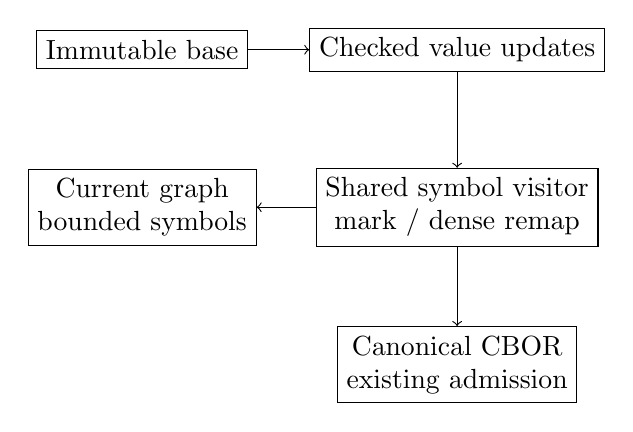
\begin{tikzpicture}[every node/.style={draw,align=center}]
\node (base) at (0,0) {Immutable base};
\node (edit) at (4,0) {Checked value updates};
\node (compact) at (4,-2) {Shared symbol visitor\\mark / dense remap};
\node (next) at (0,-2) {Current graph\\bounded symbols};
\node (wire) at (4,-4) {Canonical CBOR\\existing admission};
\draw[->] (base)--(edit);\draw[->] (edit)--(compact);
\draw[->] (compact)--(next);\draw[->] (compact)--(wire);
\end{tikzpicture}

\end{document}
